\section{Genomförande}
Modellprovaren skrevs i prolog då det är ett lämpligt programmeringsspråk för bevissökning. De befintliga reglerna för CTL implementerades. Vissa av reglerna kräver variabelt antal premisser och detta måste hanteras av programmet.

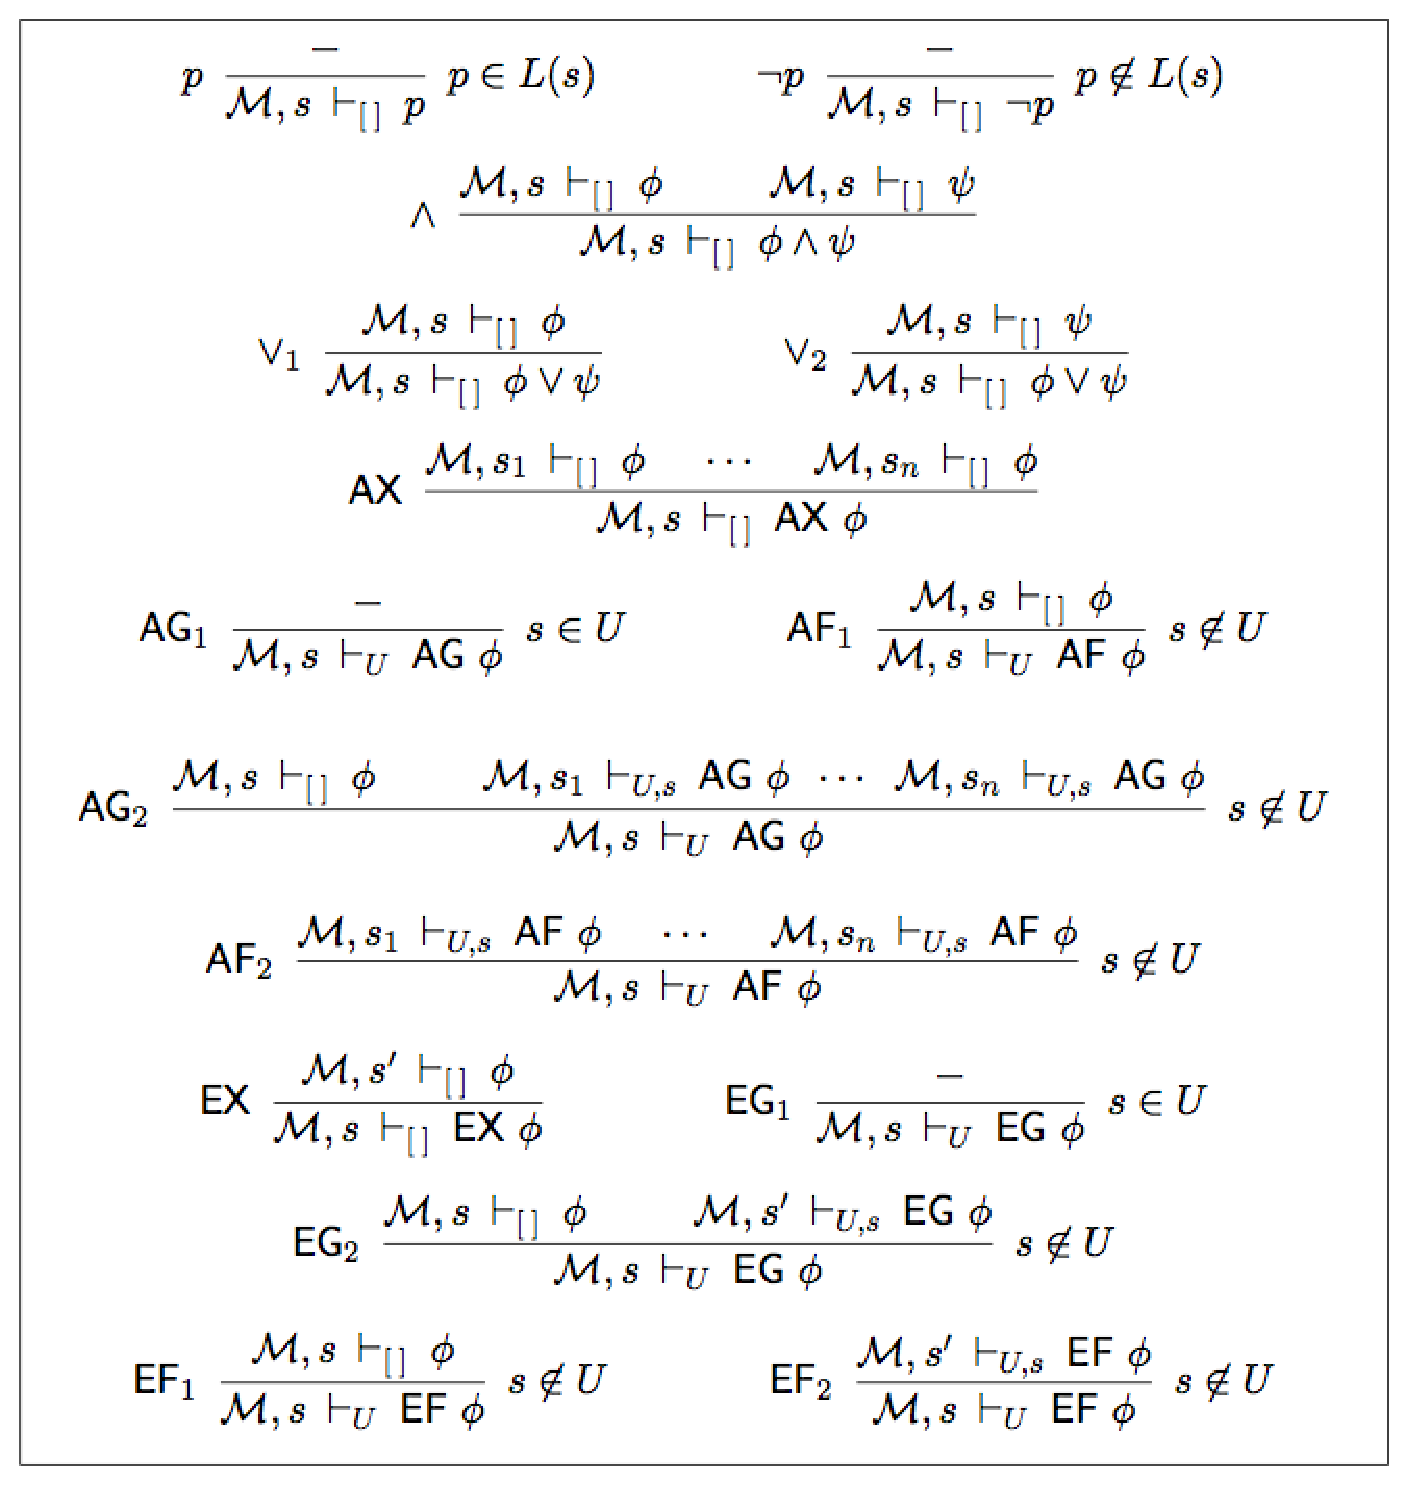
\includegraphics[width=\textwidth]{formulas.eps}

För att kunna testa modellprovaren fanns flertalet tester att tillgå som bestod av en liststruktur för att beskriva tillståndens egenskaper och grannar, detta beskrivs tydligare under Modell.
Programmet skrevs så att en funktion “check” anropades med följande inparametrar:

\begin{center}
\begin{minipage}{0.75\textwidth}

\texttt{check(T, L, S, U, F)}

\texttt{T - Alla tillstånd och dess grannar i listform}

\texttt{L - Lista över egenskaper i varje tillstånd}

\texttt{S - Aktuellt tillstånd}

\texttt{U - Lista för besökta tillstånd}

\texttt{F - CTL formel som ska testas}

\end{minipage}
\end{center}

Check skrevs så att den med pattern matching kan matchas mot alla de regler som skulle implementeras. De matchades på följande sätt: \texttt{X}, \texttt{neg(X)}, \texttt{and(F,G)}, \texttt{or(F,G)}, \texttt{ax(X)}, \texttt{ag(X)}, \texttt{ex(X)}, \texttt{eg(X)}, \texttt{ef(X)}.

Nedan följer ett utrag ur programkoden för kontroll av \texttt{ef(X)}:

\begin{center}
\begin{minipage}{0.6\textwidth}

\begin{verbatim}
% EF1:
check(T, L, S, U, ef(X)) :-
	not(member(S,U)),
	check(T, L, S, [], X).
\end{verbatim}


\begin{verbatim}
% EF2:
check(T, L, S, U, ef(X)) :-
	not(member(S,U)),	
	member([S,Srest],T),
	echeck(T, L, Srest, [S|U], ef(X)).
\end{verbatim}


\end{minipage}
\end{center}

Då check stötte på \texttt{ef(X)} försökte den först med implementationen EF1 och sedan om den evaluerades till false försökte den med EF2.